\begin{figure*}[t]
  \centering
  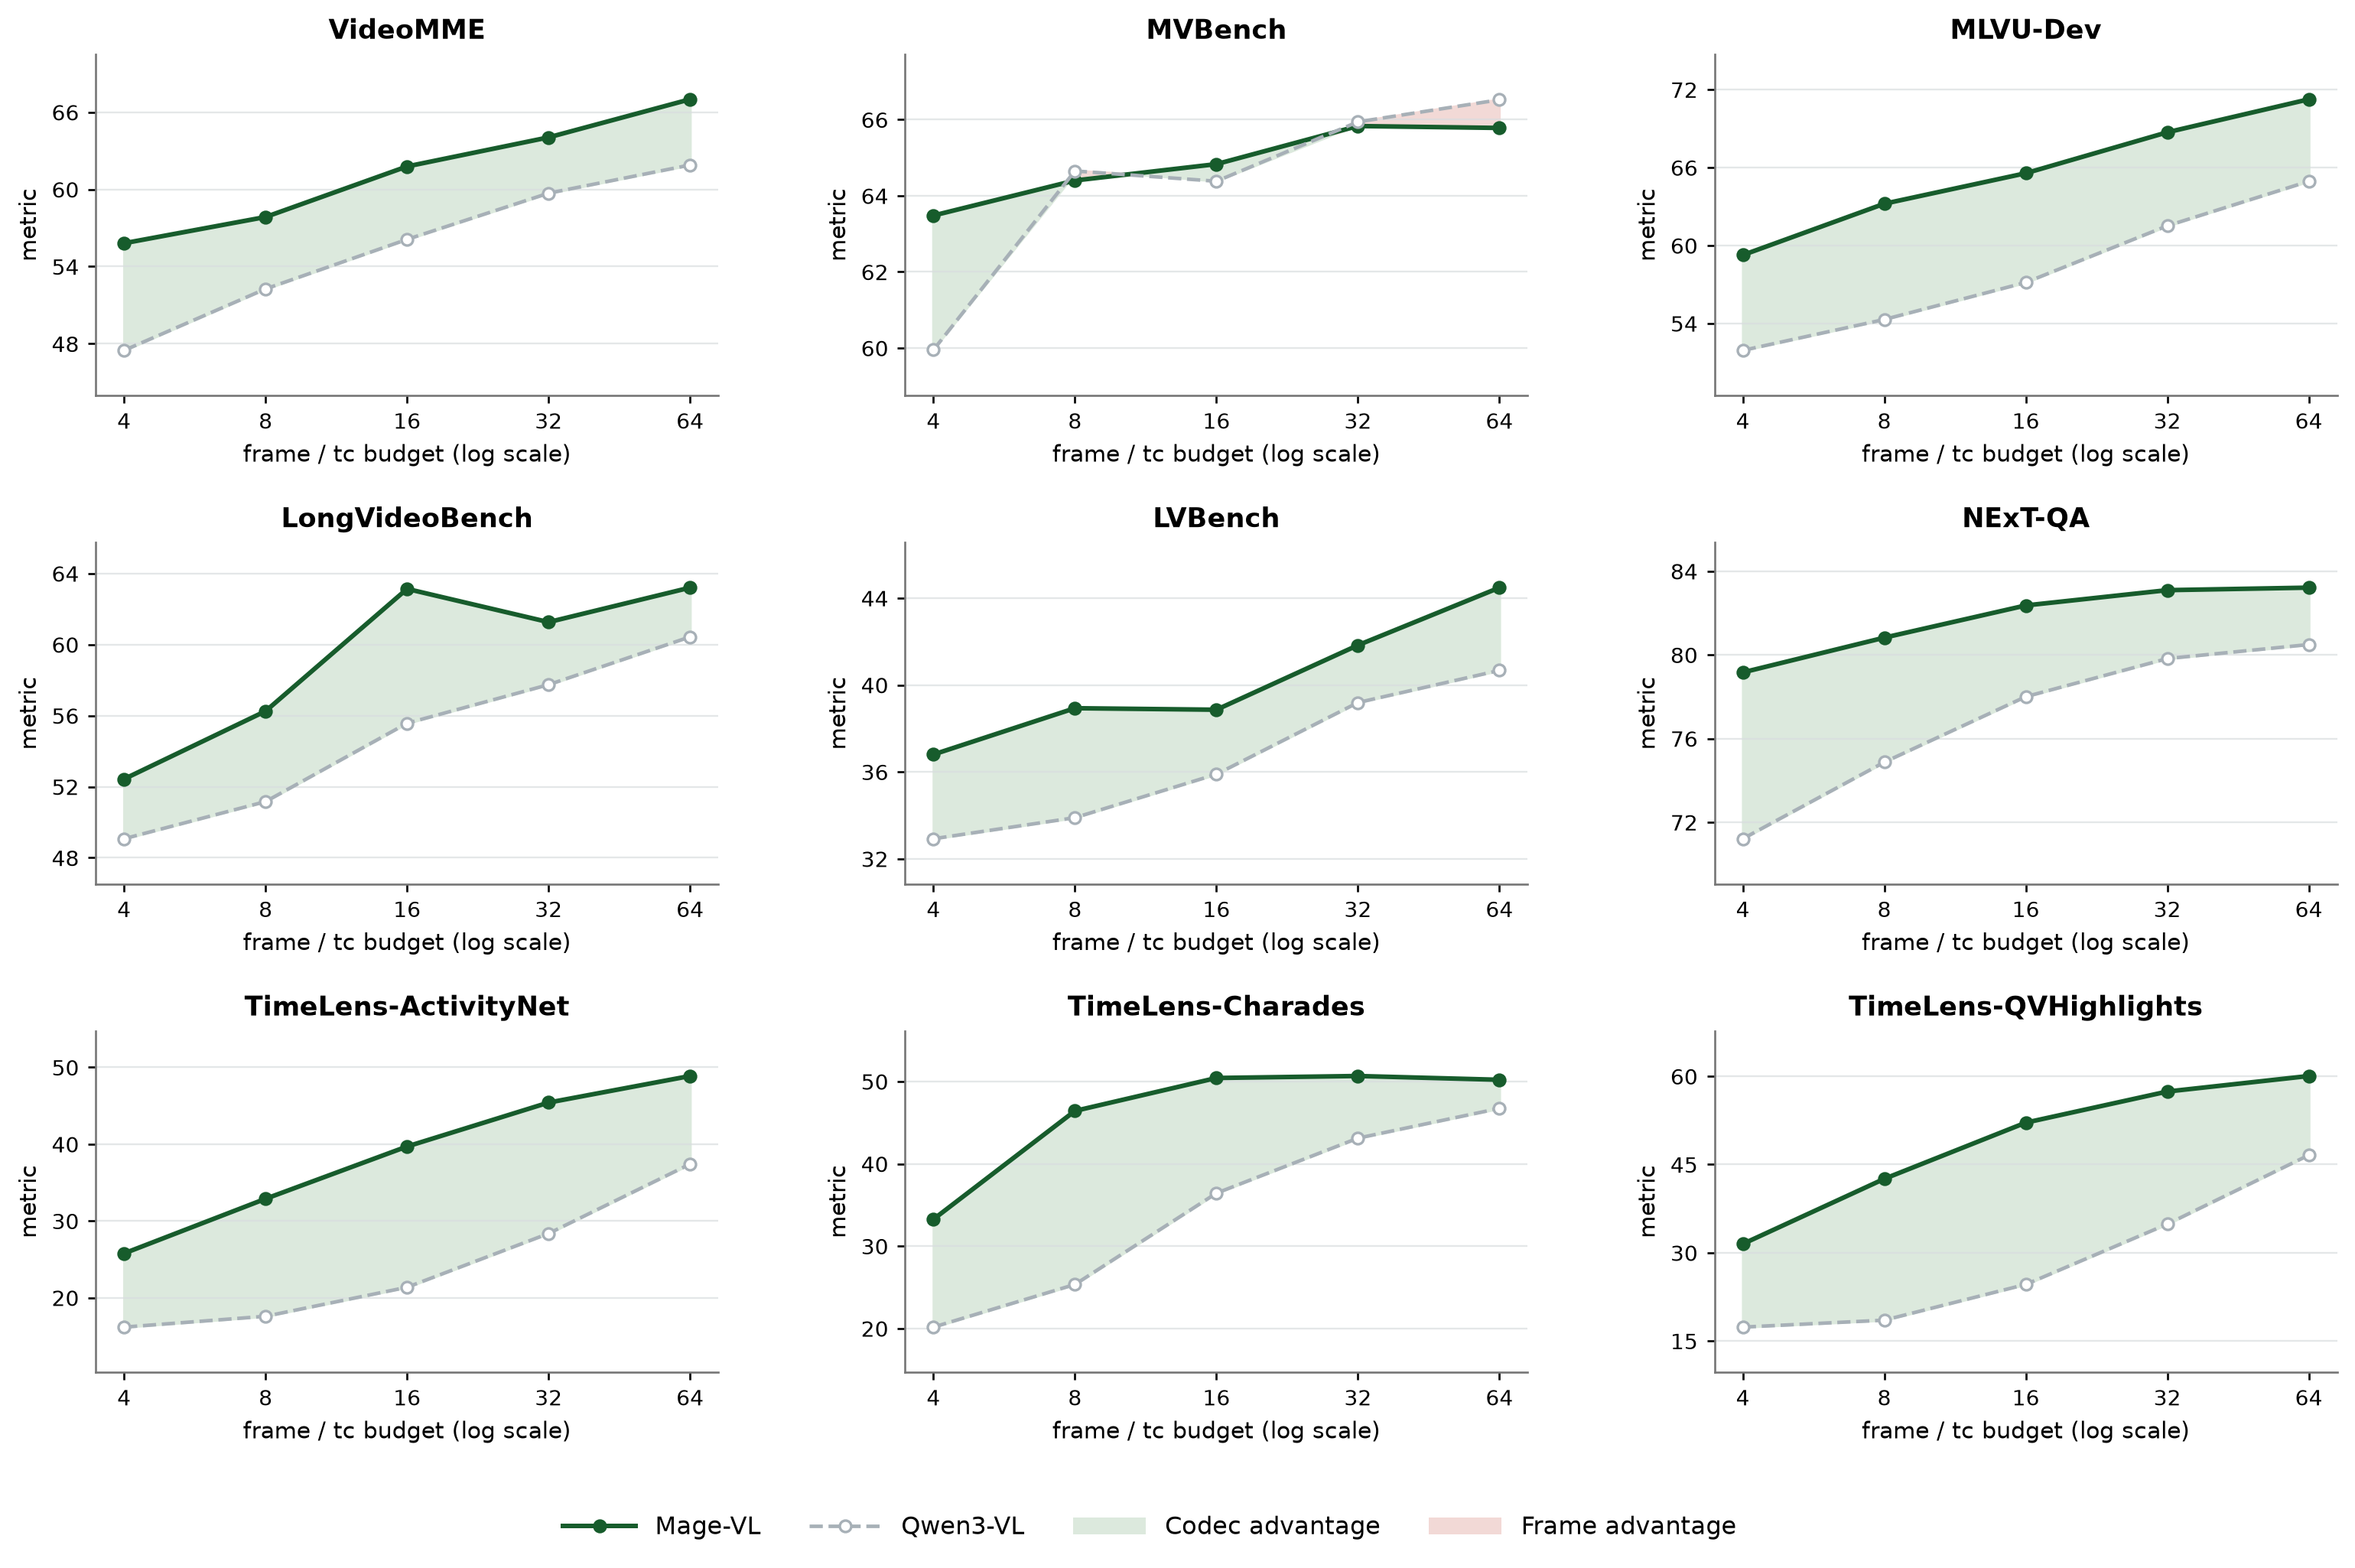
\includegraphics[width=\textwidth]{figures/tc_vs_frame_3x3.png}
  \caption{\textbf{Codec inputs versus uniform frame sampling across input budgets.}
  Frame-$N$ uses $N$ uniformly sampled RGB frames, whereas tc-$N$ targets $N$ codec canvases constructed from $8N$ source frames. Shaded regions highlight the performance gain of codec-native tokenization.}
  \label{fig:tc_vs_frame_scaling}
\end{figure*}
